\documentclass[border=10pt]{standalone}
\usepackage{pgfplots}
\pgfplotsset{compat=1.8}
\newcommand{\gt}{\ensuremath >}
\newcommand{\lt}{\ensuremath <}
\begin{document}
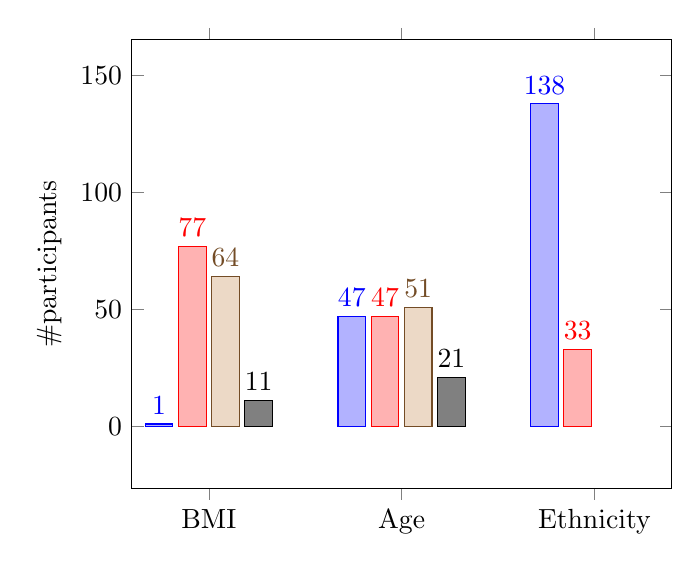
\begin{tikzpicture}
  \begin{axis}[
    ybar,
    enlargelimits=0.20,
    legend style={at={(0.5,-0.15)},
    anchor=north,legend columns=-1},
    ylabel={\#participants},
    symbolic x coords={BMI, Age, Ethnicity},
    xtick=data,
    nodes near coords,
    nodes near coords align={vertical},
    ]
    \addplot coordinates {(BMI,1) (Age,47) (Ethnicity,138)};
    \addplot coordinates {(BMI,77) (Age,47) (Ethnicity,33)};
    \addplot coordinates {(BMI,64) (Age,51) };
    \addplot coordinates {(BMI,11) (Age,21) };
    % \legend{used,understood,not understood}
  \end{axis}
\end{tikzpicture}

\newcounter{groupcount}
\pgfplotsset{
draw group line/.style n args={5}{
after end axis/.append code={
\setcounter{groupcount}{0}
\pgfplotstableforeachcolumnelement{#1}\of\datatable\as\cell{%
\def\temp{#2}
\ifx\temp\cell
\ifnum\thegroupcount=0
\stepcounter{groupcount}
\pgfplotstablegetelem{\pgfplotstablerow}{[index]0}\of\datatable
\coordinate [yshift=#4] (startgroup) at (axis cs:\pgfplotsretval,0);
\else
\pgfplotstablegetelem{\pgfplotstablerow}{[index]0}\of\datatable
\coordinate [yshift=#4] (endgroup) at (axis cs:\pgfplotsretval,0);
\fi
\else
\ifnum\thegroupcount=1
\setcounter{groupcount}{0}
\draw [
shorten >=-#5,
shorten <=-#5
] (startgroup) -- node [anchor=north] {#3} (endgroup);
\fi
\fi
}
\ifnum\thegroupcount=1
\setcounter{groupcount}{0}
\draw [
shorten >=-#5,
shorten <=-#5
] (startgroup) -- node [anchor=north] {#3} (endgroup);
\fi
}
}
}
\makeatother

\pgfplotstableread{
1	1
2	77
3	64
4	11
5	47
6	47
7	51
8	21
9	138
10	33

}\datatable

% 
% \begin{tikzpicture}
%   \begin{axis}[
%     ylabel=label,
%     xtick=data,
%     xticklabels={$\le 21$,22 - 30,31 - 40,$\gt 40$,$\le 40$,41 - 50,51 - 60,$\gt 60$,MA,NHW},
%     x tick label style={rotate=90,anchor=east},
%     enlarge y limits=false,
%     enlarge x limits=0.1,
%     ymin=0,ymax=100,
%     ybar stacked,
%     bar width=10pt,
%     legend style={
%     font=\footnotesize,
%     cells={anchor=west},
%     legend columns=5,
%     at={(0.3,-0.20)},
%     anchor=north,
%     /tikz/every even column/.append style={column sep=0.2cm}
%     },
%     ]
%     \addplot table[x index=0,y index=1] \datatable;
%     % \addplot table[x index=0,y index=2] \datatable;
%     % \addplot table[x index=0,y index=3] \datatable;
%     \legend{Far,Near,Here}
%   \end{axis}
%   \begin{axis}[
%     ylabel=label,
%     xtick=data,
%     xticklabels={$\le 21$,22 - 30,31 - 40,$\gt 40$,$\le 40$,41 - 50,51 - 60,$\gt 60$,MA,NHW},
%     x tick label style={rotate=90,anchor=east},
%     enlarge y limits=false,
%     enlarge x limits=0.1,
%     ymin=0,ymax=100,
%     legend style={
%     font=\footnotesize,
%     cells={anchor=west},
%     legend columns=5,
%     at={(0.71,-0.20)},
%     anchor=north,
%     /tikz/every even column/.append style={column sep=0.2cm}
%     },
%     draw group line={[index]6}{1}{BMI}{-10ex}{7pt},
%     draw group line={[index]6}{2}{Age}{-10ex}{7pt},
%     draw group line={[index]6}{3}{Ethnicity}{-10ex}{7pt}
%     ]
%     % \addplot+[forget plot,only marks,mark=*] table[x index=0,y index=4, restrict x to domain=0:4] \datatable;
%     % \addplot+[forget plotonly marks,mark=*] table[x index=0,y index=4, restrict x to domain=5:8] \datatable;
%     % \addplot+ table[x index=0,y index=4, restrict x to domain=9:10] \datatable;
%     % \legend{There}
%   \end{axis}
% \end{tikzpicture}

\end{document}
